\documentclass[11pt,class=report,crop=false]{standalone}
\usepackage[screen]{../python}

\begin{document}

%====================================================================
\chapitre{Réseau de neurones}
%====================================================================

\insertvideo{MfptsiyntVo}{partie 5.1. Un neurone}

\insertvideo{xccdozKWAe8}{partie 5.2. Théorie avec un neurone}

\insertvideo{CeRlYwIscJQ}{partie 5.3. Plusieurs neurones}

\insertvideo{2JnyMQpaRMU}{partie 5.4. Théorie avec plusieurs neurones}

\insertvideo{ReLK3O4wyuA}{partie 5.5. Théorème d'approximation universelle}


\objectifs{Le cerveau humain est composé de plus de $80$ milliards de neurones. Chaque neurone reçoit des signaux électriques d'autres neurones et réagit en envoyant un nouveau signal à ses neurones voisins.
Nous allons construire des réseaux de neurones artificiels. Dans ce chapitre, nous ne chercherons pas à expliciter une manière de déterminer dynamiquement les paramètres du réseau de neurones, ceux-ci seront fixés ou bien calculés à la main.}


%%%%%%%%%%%%%%%%%%%%%%%%%%%%%%%%%%%%%%%%%%%%%%%%%%%%%%%%%%%%%%%%%%%%%
\section{Perceptron}

%--------------------------------------------------------------------
\subsection{Perceptron linéaire}

\index{perceptron!lineaire@linéaire}

Le principe du perceptron linéaire est de prendre des valeurs en entrées, de faire un calcul simple et de renvoyer une valeur en sortie. Les calculs dépendent de paramètres propres à chaque perceptron.

\myfigure{1}{
	\tikzinput{fig_neurones_01}
}



Le calcul effectué par un perceptron se décompose en deux phases : un calcul par une fonction linéaire $f$, suivi d'une fonction d'activation $\phi$.

\myfigure{1}{
	\tikzinput{fig_neurones_02}
}


Détaillons chaque phase.
\begin{itemize}
  \item \textbf{Partie linéaire.} Le perceptron est d'abord muni de \defi{poids}\index{poids} $a_1,\ldots,a_n$
  qui déterminent une fonction linéaire 
  $$f(x_1,\ldots,x_n) = a_1 x_1 + a_2 x_2 + \cdots + a_n x_n.$$
  \item \textbf{Fonction d'activation.}\index{fonction d'activation} La valeur renvoyée par la fonction linéaire $f$ est ensuite composée par une fonction d'activation $\phi$.
  
  \item \textbf{Sortie.} La valeur de sortie est donc $\phi(a_1 x_1 + a_2 x_2 + \cdots + a_n x_n)$.
\end{itemize}

Dans ce chapitre, la fonction d'activation sera (presque) toujours la fonction marche de Heaviside :
$$\begin{cases}
H(x) = 1 & \text{ si } x \ge 0, \\
H(x) = 0  & \text{ si } x < 0. \\
\end{cases}$$

\myfigure{1}{
	\tikzinput{fig_neurones_04}
}



Voici ce que fait un perceptron linéaire de poids $a_1,\ldots,a_n$ et de fonction d'activation la fonction marche de Heaviside :

\myfigure{0.8}{
	\tikzinput{fig_neurones_03}
}


On peut donc définir ce qu'est un perceptron. Un \defi{perceptron linéaire} à $n$ variables et de fonction d'activation la fonction marche de Heaviside est la donnée de $n$ coefficients réels $a_1,\ldots,a_n$ auxquels est associée la fonction $F : \Rr \to \Rr$ définie par $F = H \circ f$, c'est-à-dire :
$$\begin{cases}
F(x_1,\ldots,x_n) = 1 & \text{ si } a_1 x_1 + a_2 x_2 + \cdots + a_n x_n \ge 0, \\
F(x_1,\ldots,x_n) = 0  & \text{ sinon.} \\
\end{cases}$$



\begin{exemple}

Voici un perceptron à deux entrées. Il est défini par les poids $a=2$ et $b=3$.

\myfigure{0.8}{
	\tikzinput{fig_neurones_05}
}


\begin{itemize}
  \item \textbf{Formule.}
  
Notons $x$ et $y$ les deux réels en entrée.
La fonction linéaire $f$ est donc 
$$f(x,y) = 2x+3y.$$

La valeur en sortie est donc :
$$\begin{cases}
F(x,y) = 1 & \text{ si } 2x+3y \ge 0 \\
F(x,y) = 0  & \text{ sinon.} \\
\end{cases}$$

\myfigure{0.8}{
	\tikzinput{fig_neurones_06}
}

  \item \textbf{\'Evaluation.} 
  Utilisons ce perceptron comme une fonction. Que renvoie le perceptron pour la valeur d'entrée $(x,y) = (4,-1)$ ?
On calcule $f(x,y) = 2x+3y = 5$. Comme $f(x,y)\ge0$, alors la valeur de sortie est donc $F(x,y) = 1$.

	Recommençons avec $(x,y) = (-3,1)$. Cette fois $f(x,y) = -3 < 0$ donc $F(x,y) = 0$.
	
	L'entrée $(x,y) = (6,-4)$ est \og{}à la limite\fg{} car $f(x,y)=0$ ($0$ est l'abscisse critique pour la fonction marche de Heaviside).
	On a $F(x,y) = 1$.

  \item \textbf{Valeurs de la fonction.}
  
  La fonction $F$ prend seulement deux valeurs : $0$ ou $1$. La frontière correspond aux points $(x,y)$ tels que
  $f(x,y)=0$, c'est-à-dire à la droite $2x+3y=0$.  
  Pour les points au-dessus de la droite (ou sur la droite) la fonction $F$ prend la valeur $1$ ;
  pour les points en-dessous de la droite, la fonction $F$ vaut $0$.
  
\myfigure{0.8}{
	\tikzinput{fig_neurones_07}
}  
  
\end{itemize}
\end{exemple}

\textbf{Notation.}

Nous représentons un perceptron par une forme plus condensée : 
sous la forme d'un \defi{neurone}, avec des poids sur les arêtes d'entrées. 
Nous précisons en indice la fonction d'activation utilisée  $\phi$.
Si le contexte est clair cette mention est omise.

\myfigure{0.7}{
	\tikzinput{fig_neurones_08}
}  
  
Voici le neurone à deux variables de l'exemple précédent.
\myfigure{0.7}{
	\tikzinput{fig_neurones_09}
}  

\begin{exemple}
Voici deux catégories de points : des ronds bleus et des carrés rouges. Comment trouver un perceptron qui les sépare ?

\myfigure{0.7}{
	\tikzinput{fig_neurones_10}
} 

Il s'agit donc de trouver les deux poids $a$ et $b$ d'un perceptron, dont la fonction associée
$F$ vérifie $F(x,y)=1$ pour les coordonnées des carrés et $F(x,y)=0$ pour les ronds.

\myfigure{0.7}{
	\tikzinput{fig_neurones_11}
} 

Trouvons une droite qui les sépare. Par exemple, la droite d'équation $4x-y=0$ sépare les ronds des carrés. On définit donc le neurone avec les poids $a=4$ et $b=-1$.
Si $(x,y)$ sont les coordonnées d'un carré alors on a bien $F(x,y)=1$ et pour un rond $F(x,y)=0$.

\begin{center}
\begin{minipage}{0.35\textwidth}
\myfigure{0.5}{
\tikzinput{fig_neurones_12}
}
\end{minipage}
\begin{minipage}{0.45\textwidth}
\myfigure{0.6}{
\tikzinput{fig_neurones_13}
}
\end{minipage}
\end{center}


\end{exemple}


%--------------------------------------------------------------------
\subsection{Biais -- Perceptron affine}

Pour l'instant notre perceptron à deux entrées sépare le plan en deux parties selon une droite passant par l'origine.
Nous allons plus loin avec le \defi{perceptron affine}.\index{perceptron!affine@affine}

On modifie la définition du perceptron, sans changer le nombre d'entrées, mais en ajoutant un poids supplémentaire.
Dans le cas de $n$ entrées il y  a donc $n+1$ \defi{poids} : 
\begin{itemize} 
  \item les \defi{coefficients} $a_1,\ldots,a_n \in \Rr$,
  \item et le \defi{biais}\index{biais} $a_0 \in \Rr$,
\end{itemize}
qui définissent la fonction affine :
$$f(x_1,\ldots,x_n) = a_1 x_1 + a_2 x_2 + \cdots + a_n x_n + a_0.$$
Comme auparavant, ce calcul est suivi de la fonction d'activation.


\myfigure{0.7}{
	\tikzinput{fig_neurones_14}
}

On représente le neurone avec une nouvelle arête, pondérée par le biais. L'arête  est terminée par un rond pour signifier que cela ne correspond pas à une entrée.

\myfigure{0.6}{
	\tikzinput{fig_neurones_15}
}


Dans le cas de deux entrées, les poids sont trois réels $a,b$ (les coefficients) et $c$ (le biais).
\myfigure{0.6}{
	\tikzinput{fig_neurones_16}
}

La fonction $f : \Rr^2 \to \Rr$ est la fonction affine $f(x,y) =ax+by+c$.
Si la fonction d'activation est la fonction marche de Heaviside, alors le perceptron affine définit une fonction $F : \Rr^2 \to \Rr$ par la formule :
$$\begin{cases}
F(x,y) = 1 & \text{ si } ax+by+c \ge 0 \\
F(x,y) = 0  & \text{ sinon.} \\
\end{cases}$$


Un perceptron affine à deux entrées sépare donc le plan en deux parties, la frontière étant la droite d'équation $ax+by+c=0$.
D'un côté de cette droite la fonction $F$ vaut $1$, de l'autre elle vaut $0$.

\myfigure{0.7}{
	\tikzinput{fig_neurones_17}
}

\begin{center}
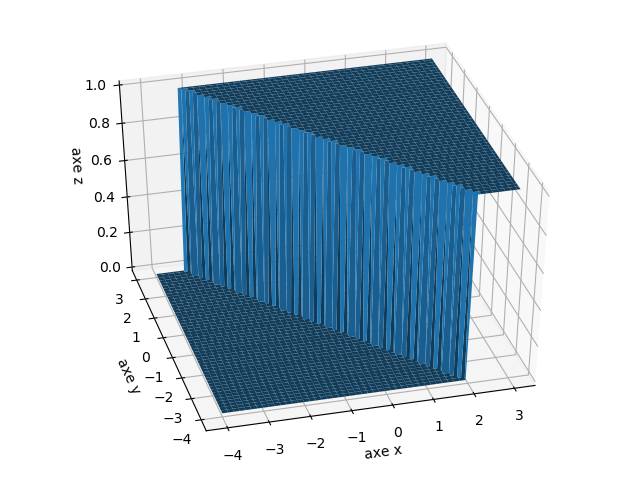
\includegraphics[scale=\myscale,scale=0.7]{figures/neurones-surface-4}
\end{center}



\begin{exercicecours}
Trouver un perceptron qui distingue les carrés des ronds.
\myfigure{0.7}{
	\tikzinput{fig_neurones_18}
}
\end{exercicecours}


\bigskip

Il n'est pas toujours possible de répondre à une question seulement par \og{}oui\fg{} ou \og{}non\fg{}.
Pour y remédier, on peut changer de fonction d'activation en utilisant par exemple la fonction sigmoïde $\sigma$.
Dans ce cas, à chaque point du plan, on associe, non plus $0$ ou $1$, mais une valeur entre $0$ et $1$. 


Ce nombre peut correspondre à un degré de certitude. Par exemple avec une question \og{}Est-ce que cette photo est un chat ?\fg{}, si 
la sortie vaut $0.8$, cela signifie \og{}c'est bien un chat avec $80\%$ de certitude\fg{}. Si la sortie vaut $0.1$ alors ce n'est probablement pas un chat.

Voici un neurone à deux entrées muni de la fonction d'activation sigmoïde définie par $\sigma(x) = \frac{1}{1+e^{-x}}$.

\begin{center}
\begin{minipage}{0.45\textwidth}
\myfigure{0.5}{
\tikzinput{fig_neurones_20}
}
\end{minipage}
\begin{minipage}{0.45\textwidth}
\myfigure{0.6}{
\tikzinput{fig_neurones_19}
}
\end{minipage}
\end{center}

\begin{center}
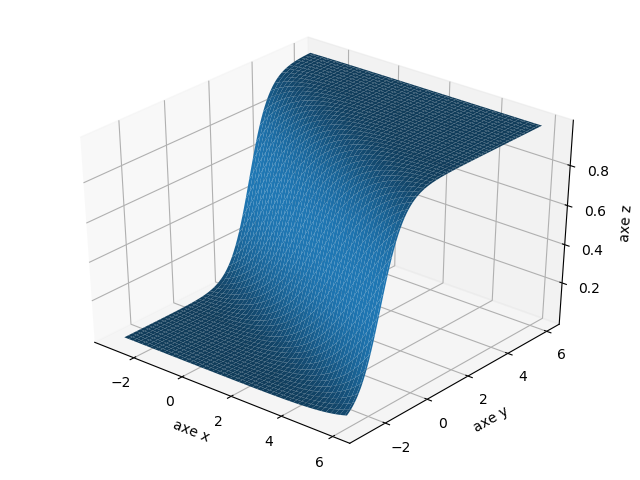
\includegraphics[scale=\myscale,scale=0.75]{figures/neurones-surface-3}
\end{center}


\begin{exemple}
Voici les données (fictives) de la répartition des hommes et des femmes selon leur taille et leur poids.
  
\myfigure{0.7}{
	\tikzinput{fig_neurones_21}
}  


Problème : la taille et le poids d'une personne étant donnés, trouver un perceptron qui réponde à la question \og{}Cette personne est-elle un homme ou une femme ?\fg{}.

Au vu de la superposition des zones, il n'est pas possible de répondre avec certitude.  On construit donc un perceptron selon les idées suivantes :
\begin{itemize}
  \item on trace une droite qui sépare au mieux les hommes des femmes, par exemple ici la droite qui passe par les points $A(1.40,52)$ et $B(2.06,93)$ d'équation approchée $y=68x-44$ où $(x,y)=(t,p)$ représente la taille et le poids ;

  \item on choisit la fonction d'activation sigmoïde.
\end{itemize}
Ce qui nous permet de définir le perceptron suivant avec $a=68$, $b=-1$ et $c=-44$.

\begin{center}
\begin{minipage}{0.35\textwidth}
\myfigure{0.4}{
\tikzinput{fig_neurones_22}
}
\end{minipage}
\begin{minipage}{0.45\textwidth}
\myfigure{0.7}{
\tikzinput{fig_neurones_23}
}
\end{minipage}
\end{center}

Maintenant pour un couple donné $(t,p)$, le perceptron associe une valeur $F(t,p) \in [0,1]$.
Si $F(t,p)$ est proche de $0$ alors la personne est probablement un homme, si $F(t,p)$ est proche de $1$ c'est probablement une femme.


Exemple : une personne mesurant $1.77$\,m et pesant $79$\,kg est-elle plutôt un homme ou une femme ? On calcule $f(1.77,79)=-2.64$ où $f(x,y)=ax+by+c$.
Puis on calcule $F(1.77,79) = \sigma(-2.64) \simeq 0.07$. Selon notre modèle cette personne est probablement un homme (car la valeur de $F$ est proche de $0$).

Autre exemple : $(t,p)=(1.65,67)$. On calcule $F(1.65,67) \simeq 0.76$.
Une personne mesurant $1.65$m et pesant $67$kg est probablement une femme (car la valeur de $F$ est plus proche de $1$ que de $0$).

Malgré les données fictives, cet exemple met en évidence le problème de la superposition et de l'utilité d'avoir une sortie plus riche que  \og{}oui\fg{} ou \og{}non\fg{}. On peut aussi discuter de la pertinence de la frontière, car la séparation par une droite ne semble pas la mieux adaptée.  En fait, le poids varie en fonction du carré de la taille (les zones ont une forme de parabole). 
\end{exemple}




Plus généralement un \defi{perceptron affine} à $n$ entrées est la donnée de $n+1$ poids $a_0,a_1,\ldots,a_n \in \Rr$
et d'une fonction d'activation $\phi$ qui définissent une fonction $F : \Rr^n \to \Rr$
par la formule :
$$F(x_1,\ldots,x_n) = \phi(a_1 x_1 + \cdots + a_n x_n + a_0).$$

\begin{exemple}
Dans le système de couleurs RGB (\emph{red, green, blue}), une couleur est déterminée par trois réels $r,g,b \in [0,1]$.
Le \og{}vrai\fg{} rouge est codé par $(1,0,0)$, mais bien sûr des couleurs proches sont aussi des nuances de rouge.
On représente toutes les couleurs par un \og{}cube de couleurs\fg{}, chaque point du cube représente le code $(r,g,b)$ d'une couleur.

\myfigure{0.8}{
\tikzinput{fig_neurones_24}
}

On décide (un peu arbitrairement) que toute couleur située dans la zone du coin $(1,0,0)$ de la figure ci-dessus est une nuance de rouge.

Problème : trouver un perceptron qui répond à la question \og{}Cette couleur est-elle une nuance de rouge ?\fg{}.

Solution. On considère que la zone est délimitée par le plan passant par les points $A(\frac12,0,0)$, $B(1,\frac12,0)$ et $C(1,0,\frac12)$ et les plans des faces du cube.
Une équation de ce plan est $2x-2y-2z-1 = 0$ où en fait $(x,y,z)=(r,g,b)$.
Le perceptron qui répond à la question est donc :

\myfigure{0.7}{
\tikzinput{fig_neurones_25}
}

La fonction $F$ associée, vérifie que $F(r,g,b) = 1$ pour les points de la zone des rouges et $F(r,g,b)=0$ sinon.
 
\end{exemple}



%%%%%%%%%%%%%%%%%%%%%%%%%%%%%%%%%%%%%%%%%%%%%%%%%%%%%%%%%%%%%%%%%%%%%
\section{Théorie du perceptron}

%--------------------------------------------------------------------
\subsection{OU, ET, OU exclusif}

\textbf{OU.}
Un \defi{booléen} est une variable qui peut prendre soit la valeur \og{}vrai\fg{}, soit la valeur \og{}faux\fg{}. 
Dans la pratique, on associe $1$ à \og{}vrai\fg{} et $0$ à \og{}faux\fg. \`A partir de deux booléens $x$ et $y$, on peut associer un nouveau booléen
\og{}$x$ OU $y$\fg{} qui est vrai lorsque $x$ est vrai ou $y$ est vrai.
 
Graphiquement, on représente toutes les configurations associées à \og{}$x$ OU $y$\fg{} par un diagramme. Un rond bleu en position $(x,y)$ signifie que \og{}$x$ OU $y$\fg{} est faux (le résultat vaut $0$), un carré rouge que \og{}$x$ OU $y$\fg{} est vrai (le résultat vaut $1$).

\myfigure{1}{
\tikzinput{fig_neurones_26}
}


Peut-on réaliser l'opération \og{}$x$ OU $y$\fg{} par un perceptron ? 
Oui ! Cela revient à séparer les ronds bleus des carrés rouges.
C'est possible avec le perceptron de poids $a=1$, $b=1$, $c=-1$.
Par exemple, si $x=0$ et $y=1$ alors, on calcule $1\cdot0+1\cdot1-1 = 0 \ge0$. Composée avec la fonction marche de Heaviside, la fonction $F(x,y)$
définie par le perceptron renvoie dans ce cas $1$ (\og{}vrai\fg{}).
Si $x=0$ et $y=0$, alors $1\cdot0+1\cdot0-1 = -1 <0$ et $F(x,y)=0$ (\og{}faux\fg{}).

\begin{center}
\begin{minipage}{0.35\textwidth}
\myfigure{0.4}{
\tikzinput{fig_neurones_27}
}
\end{minipage}
\begin{minipage}{0.45\textwidth}
\myfigure{0.7}{
\tikzinput{fig_neurones_28}
}
\end{minipage}
\end{center}


\bigskip
\textbf{ET.}
On peut également réaliser l'opération \og{}$x$ ET $y$\fg{} (qui renvoie \og{}vrai\fg{} uniquement si $x$ et $y$ sont vrais) en choisissant les poids $a=1$, $b=1$, $c=-2$.

\begin{center}
\begin{minipage}{0.35\textwidth}
\myfigure{0.4}{
\tikzinput{fig_neurones_29}
}
\end{minipage}
\begin{minipage}{0.45\textwidth}
\myfigure{0.7}{
\tikzinput{fig_neurones_30}
}
\end{minipage}
\end{center}

\begin{remarque*}
D'un point de vue numérique, si on considère des valeurs réelles pour $x$ et $y$, notre perceptron \og{}ET\fg{} n'est pas numériquement très stable.
Par exemple avec $x=0.9$ et $y=0.9$, on calcule $x+y-2=-0.2$ et la sortie est $0$, mais comme $x$ et $y$ sont proches de $1$, on aimerait que la sortie soit $1$.
Il suffit de changer un peu les paramètres : prenons $a=1$, $b=1$ et $c=-1.5$, alors $x+y-1.5=0.3$ et cette fois la sortie est $1$.
\end{remarque*}

\bigskip
\textbf{OU exclusif.}\index{ou exclusif}
Le ou exclusif, noté \og{}$x$ OUex $y$\fg{} est vrai lorsque $x$ ou $y$ est vrai, mais pas les deux en même temps. Le ou exclusif est-il réalisable par un perceptron ? Cette fois la réponse est non !

\myfigure{1}{
\tikzinput{fig_neurones_31}
}


\begin{proposition}
Il n'existe pas de perceptron (affine, à deux entrées et de fonction d'activation la fonction marche de Heaviside) qui réalise le \og{}ou exclusif\fg{}.
\end{proposition}

Nous sommes convaincus géométriquement qu'il n'existe pas de droite qui sépare les ronds bleus des carrés rouges. Nous allons le prouver par un petit calcul.

\begin{proof}
Nous raisonnons par l'absurde en supposant qu'un tel perceptron existe. Nous cherchons une contradiction. 
Soit $a_1=a,a_2=b,a_0=c$ les coefficients.

\begin{center}
\begin{minipage}{0.35\textwidth}
\myfigure{0.4}{
\tikzinput{fig_neurones_32}
}
\end{minipage}
\begin{minipage}{0.45\textwidth}
\myfigure{0.6}{
\tikzinput{fig_neurones_33}
}
\end{minipage}
\end{center}

\begin{itemize}
  \item Pour $(x,y)=(1,0)$, on doit avoir $ax+by+c\ge0$ (car après avoir composé avec la fonction d'activation le résultat doit être $1$), 
  donc 
  \begin{equation}
  \label{eq:neur1}
  a+c \ge 0.
  \end{equation}
  \item De même pour $(x,y)=(0,1)$, on doit avoir $ax+by+c\ge0$, ce qui donne :
  \begin{equation}
  \label{eq:neur2}
  b+c \ge 0.
  \end{equation}
  \item Pour $(0,0)$ et $(1,1)$, on a $ax+by+c<0$, ce qui implique :
  \begin{equation}
  \label{eq:neur3}
  c<0,
  \end{equation}  
  \begin{equation}
  \label{eq:neur4}
  a+b+c<0.
  \end{equation}
\end{itemize}

Si on additionne les inégalités (\ref{eq:neur1}) et (\ref{eq:neur2}), on obtient $a+b+2c\ge0$. Par l'inégalité (\ref{eq:neur3}) on a $-c>0$. Donc en ajoutant $-c$ à l'inégalité $a+b+2c\ge0$, on obtient $a+b+c>0$. Ce qui contredit l'inégalité  (\ref{eq:neur4}).

Conclusion : il ne peut exister trois réels $a,b,c$ pour définir un perceptron réalisant le \og{}ou exclusif\fg{}.

\end{proof}


%--------------------------------------------------------------------
\subsection{Séparation linéaire}

Nous formalisons un peu les idées de la section précédente.
Une \defi{droite} du plan $\Rr^2$ est l'ensemble des points $(x,y)$ vérifiant une équation du type $ax+by+c=0$. Un \defi{plan} de l'espace $\Rr^3$ est l'ensemble des points $(x,y,z)$ vérifiant une équation du type $ax+by+cz+d=0$.  Nous généralisons cette notion en dimension plus grande.
\begin{definition}
Un \defi{hyperplan (affine)} de $\Rr^n$ est l'ensemble des points $(x_1,\ldots,x_n)$ qui vérifient une équation du type :
$$a_1 x_1 + a_2 x_2 + \cdots + a_n x_n + a_0=0$$
où $a_1,\ldots,a_n$ sont des réels (non tous nuls) et $a_0$ est aussi un réel.
\end{definition}


Le but d'un perceptron affine est de séparer deux ensembles. Par exemple deux ensembles $A$ et $B$ du plan seront séparés par une droite, deux ensembles de l'espace sont séparés par un plan.

\begin{definition}
Deux ensembles $A$ et $B$ sont \defi{linéairement séparables} s'il existe un hyperplan qui sépare $A$ de $B$. Plus précisément, s'il existe des réels  $a_0,a_1,\ldots,a_n$ tels que $a_1 x_1 + a_2 x_2 + \cdots + a_n x_n + a_0 \ge 0$ pour tout $(x_1,\ldots,x_n) \in A$ et $a_1 x_1 + a_2 x_2 + \cdots + a_n x_n + a_0 < 0$ pour tout $(x_1,\ldots,x_n) \in B$.
\end{definition}

\myfigure{0.7}{
\tikzinput{fig_neurones_34}
}

Nous résumons ce qui précède dans le résultat suivant.
\begin{proposition}
Deux ensembles $A$ et $B$ de $\Rr^n$ sont linéairement séparables si, et seulement si, il existe un perceptron affine dont la fonction $F$ vaut $1$ sur $A$ et $0$ sur $B$.
\end{proposition}

La preuve est simple : la fonction $f$ définie par un perceptron (avant activation) est une fonction affine :
$$f(x_1,\ldots,x_n) = a_1 x_1 + a_2 x_2 + \cdots + a_n x_n + a_0.$$
Si $f(x_1,\ldots,x_n) \ge 0$, alors après activation $F(x_1,\ldots,x_n)=1$, sinon $F(x_1,\ldots,x_n)=0$.


\begin{exemple}
Réaliser \og{}$x$ OU $y$ OU $z$\fg{} revient à séparer par un plan le rond bleu des carrés rouges du cube suivant. Trouver l'équation d'un de ces plans donne donc les poids du perceptron qui conviennent. 

\begin{center}
\begin{minipage}{0.60\textwidth}
\myfigure{0.65}{
\tikzinput{fig_neurones_35}
}
\end{minipage}
\begin{minipage}{0.39\textwidth}
\myfigure{0.6}{
\tikzinput{fig_neurones_36}
}
\end{minipage}
\end{center}

\end{exemple}

\begin{exercicecours}
Trouver le perceptron qui réalise  \og{}$x$ ET $y$ ET $z$\fg{}.
\myfigure{0.7}{
\tikzinput{fig_neurones_37}
}

\end{exercicecours}

% \todo{Exercice td : comptages des cubes réalisables ou pas preuve d'un qui n'est pas réalisable.}



%--------------------------------------------------------------------
\subsection{Vocabulaire}

Résumons le vocabulaire utilisé ci-dessus ainsi que les termes anglais correspondant :

\begin{itemize}
  \item le \textbf{perceptron linéaire} ou \textbf{neurone artificiel}, a un biais qui vaut $0$, à la différence du \textbf{perceptron affine} pour lequel le biais est un réel quelconque ;
   
  \item les \textbf{poids} (\emph{weights}) ou \textbf{paramètres} sont les \textbf{coefficients} $a_1,\ldots,a_n$ auxquels s'ajoute le \textbf{biais} (\emph{bias}) (dans ce livre le biais est l'un des poids, ce qui n'est pas toujours le cas dans la littérature) ;
  
  \item un perceptron est la donnée des poids et d'une fonction d'activation ;
  
  \item chaque perceptron définit une fonction $F$ qui est la composée d'une \textbf{fonction affine} $f$ et d'une \textbf{fonction d'activation} $\phi$ ; 
  la fonction d'activation la plus utilisée dans ce chapitre est la fonction marche de Heaviside (\emph{step function}) ; 
  
  \item on utilise un perceptron lors d'une \textbf{évaluation} : pour une \textbf{entrée} (\emph{input})
  $(x_1,\ldots,x_n) \in \Rr^n$, on calcule la sortie (\emph{output}) $F(x_1,\ldots,x_n) \in \Rr$ (qui vaut $0$ ou $1$ dans le cas de la fonction marche de Heaviside).  
\end{itemize}


\myfigure{0.8}{
\tikzinput{fig_neurones_99}
}


%%%%%%%%%%%%%%%%%%%%%%%%%%%%%%%%%%%%%%%%%%%%%%%%%%%%%%%%%%%%%%%%%%%%%
\section{Réseau de neurones}

Un neurone permet de séparer l'espace en deux parties, la frontière étant linéaire (avec deux entrées c'est une droite, avec trois entrées c'est un plan\ldots). Un neurone est trop élémentaire pour résoudre nos problèmes, par exemple il ne peut réaliser le \og{}ou exclusif\fg{}. Comment faire mieux ? En connectant plusieurs neurones !

%--------------------------------------------------------------------
\subsection{Couches de neurones}

Un \defi{réseau de neurones} est la juxtaposition de plusieurs neurones, regroupés par \defi{couches}. 

\myfigure{1}{
\tikzinput{fig_neurones_38}
}



\`A un réseau de neurones on associe une fonction.
Si à la dernière couche la fonction ne contient qu'un seul neurone (voir ci-dessus), cette fonction est  
$F : \Rr^n \to \Rr$, $y = F(x_1,\ldots,x_n)$ où $(x_1,\ldots,x_n)$ est l'\defi{entrée} et $y$ est la \defi{sortie}.
Sinon (voir ci-dessous), la fonction est  
$F : \Rr^n \to \Rr^p$, $(y_1,\ldots,y_p) = F(x_1,\ldots,x_n)$ où $(x_1,\ldots,x_n) \in \Rr^n$ est l'entrée et $(y_1,\ldots,y_p)$ est la sortie.

\myfigure{1}{
\tikzinput{fig_neurones_39}
}


\begin{exemple}
Voici un réseau de neurones à deux couches : $2$ neurones (perceptrons linéaires) sur la première couche (ayant pour fonction d'activation la fonction ReLU), $1$ neurone (perceptron affine) sur la seconde couche  (de fonction d'activation $H$).

\myfigure{1}{
\tikzinput{fig_neurones_40}
}



\begin{itemize}
  \item Si $x=4$ et $y=7$ alors on calcule la sortie de chaque neurone de la première couche. Ces sorties sont les entrées du neurone de la seconde couche.
  Pour le premier neurone, on effectue le calcul $2\cdot4+(-1)\cdot7 = 1 \ge0$, le réel étant positif la fonction ReLU le garde inchangé : le premier neurone renvoie la valeur $s_1=1$. Le second neurone effectue le calcul $(-3)\cdot4+2\cdot7 = 2 \ge0$ et renvoie $s_2=2$.
  Le neurone de la couche de sortie reçoit en entrées $s_1$ et $s_2$ et effectue le calcul $4\cdot 1+5\cdot 2-1 = 13\ge0$. La fonction d'activation étant $H$, ce neurone renvoie $1$.  
  Ainsi $F(4,7)=1$.
  
  \myfigure{1}{
  \tikzinput{fig_neurones_41}
  }
  
  
  \item Si $(x,y)=(3,2)$ alors $s_1=4$, par contre $s_2=0$ car $(-3)\cdot3+2\cdot2 = -5 <0$ et la fonction ReLU renvoie $0$ (on dit que le neurone ne s'active pas). Les entrées du dernier neurone sont donc $s_1=4$ et $s_2=0$, ce neurone calcule $4\cdot 4 + 5\cdot0-1=15\ge0$ et, après la fonction d'activation, renvoie $1$. 
  Donc $F(3,2)=1$.
  
  \item Vérifier que pour $(x,y)=(\frac1{10},\frac1{10})$ le premier neurone s'active, le second ne s'active pas (il renvoie $0$) et le dernier neurone renvoie $0$. Ainsi $F(\frac1{10},\frac1{10})=0$.
\end{itemize}
\end{exemple}


\begin{remarque*}
\sauteligne
\begin{itemize}
  \item Chaque neurone est défini par ses poids et une fonction d'activation. Pour une couche donnée, on choisit toujours la même fonction d'activation. En général on choisit la même fonction d'activation pour tout le réseau, sauf peut-être pour la couche de sortie.

  \item Un neurone prend plusieurs valeurs en entrée mais ne renvoie qu'une seule valeur en sortie ! Si ce neurone est connecté à plusieurs autres neurones, il envoie la même valeur à tous.
  
  \myfigure{0.5}{
  \tikzinput{fig_neurones_42}
  }
  
  \item On peut relier un neurone à tous les neurones de la couche suivante (voir ci-dessous figure de gauche). On dit que la seconde couche  est \defi{dense} ou \defi{complètement connectée}. Mais on peut aussi choisir de ne relier que certains neurones entre eux (voir ci-dessous figure de droite). S'il n'y a pas d'arêtes du neurone $A$ vers le neurone $B$, c'est que la sortie de $A$ n'intervient pas comme entrée de $B$ (cela revient à imposer un poids nul entre ces deux neurones).
  
  \myfigure{0.8}{
  \tikzinput{fig_neurones_43}\qquad\qquad
  \tikzinput{fig_neurones_44}  
  }  
 
  
  
\end{itemize}
\end{remarque*}  
  
\begin{exercicecours}
Pour le réseau de neurones représenté ci-dessous, calculer les valeurs de sortie $(Y_1,Y_2)$ pour chacune des entrées $(x,y,z)$ suivantes :
$$(0,0,0) \quad (1,0,0) \quad (1,-1,1) \quad (3,2,1)$$

\myfigure{0.8}{
  \tikzinput{fig_neurones_45}
  } 

Trouver $(x,y,z)$ tel que $Y_2$ soit nul, mais pas $Y_1$.

Trouver $(x,y,z)$ tel que $Y_1=1$ et $Y_2=7$ (commencer par déterminer les valeurs de sorties $s_1$ et $s_2$ de la première couche).
\end{exercicecours}

%--------------------------------------------------------------------
\subsection{Exemples}


\'Etudions quelques exemples plus en détails. Au lieu de calculer la sortie $F(x,y)$ pour des valeurs données, nous allons calculer $F(x,y)$ quelque soit $(x,y)$.

\vspace*{-1ex}

\begin{exemple}
Voici un réseau de $3$ neurones : deux sur la première couche et un sur la seconde. La fonction d'activation est partout la fonction marche de Heaviside.
Combien vaut la fonction associée $F$ selon l'entrée $(x,y)$ ?

\myfigure{0.8}{
  \tikzinput{fig_neurones_46}
  } 


On commence par calculer les sorties des neurones de la première couche.
Pour le premier neurone la sortie $s_1$ dépend du signe de $-x+3y$.
Si $-x+3y \ge 0$ alors $s_1(x,y)=1$, sinon $s_1(x,y)=0$. Donc pour les points $(x,y)$ situés au-dessus de la droite d'équation $-x+3y=0$, on a $s_1(x,y)=1$.
De même pour le second neurone, on a $s_2(x,y)=1$ pour les points situés au dessus de la droite $2x+y=0$. Voir la figure ci-dessous.
  \myfigure{0.6}{
  \tikzinput{fig_neurones_47}  
  } 
On reconnaît dans le neurone de sortie un neurone qui réalise le \og{}ET\fg{}. 
C'est pourquoi l'ensemble des points pour lesquels $F$ vaut $1$ est l'intersection des deux demi-plans en lesquels $s_1$ et $s_2$ valent $1$. Ainsi $F(x,y)=1$ dans un secteur angulaire et $F(x,y)=0$ ailleurs. Voir la figure ci-dessous.

  \myfigure{0.6}{
  \tikzinput{fig_neurones_48}  
  } 

\end{exemple}

\medskip

\begin{exemple}
On reprend la même architecture que l'exemple précédent, mais en changeant les poids du neurone de sortie qui réalise cette fois l'opération \og{}OU\fg{}.

  \myfigure{0.8}{
  \tikzinput{fig_neurones_49}
  } 

L'ensemble des points pour lesquels $F$ vaut $1$ est maintenant l'union des deux demi-plans en lesquels $s_1$ et $s_2$ valent $1$.

  \myfigure{0.6}{
  \tikzinput{fig_neurones_50}  
  } 
\end{exemple}

\begin{exemple}
Voici un réseau de neurones un peu plus compliqué (la fonction d'activation est $H$ partout). 
  \myfigure{0.8}{
  \tikzinput{fig_neurones_51}
  } 

Chaque neurone de la première couche délimite un demi-plan. Ce sont les demi-plans $-x+2y\ge0$, $x+y-2\ge0$ et $-y+3\ge0$.

Le neurone de sortie est un neurone qui réalise l'opération \og{}ET\fg{} : il s'active uniquement si les trois précédents neurones sont activés.
Ainsi la sortie finale $F(x,y)$ vaut $1$ si et seulement si $(x,y)$ appartient simultanément aux trois demi-plans.

  \myfigure{0.8}{
  \tikzinput{fig_neurones_52}  
  }

\end{exemple}

\begin{exercicecours}
En utilisant les idées de l'exemple précédent et pour le dessin ci-dessous, trouver un réseau de neurones dont la fonction $F$ vaut $1$ pour la zone colorée et $0$ ailleurs.

  \myfigure{0.5}{
  \tikzinput{fig_neurones_53}  
  }


\end{exercicecours}


\begin{exemple}
On termine en comparant les fonctions produites par des réseaux ayant la même architecture, les mêmes poids mais de fonction d'activation $\phi$ différente : $H$, $\sigma$, $\tanh$ et ReLU.

  \myfigure{0.8}{
  \tikzinput{fig_neurones_51bis}  
  }

Voici les graphiques 3D obtenus pour les fonctions d'activation $H$ (comme dans l'exemple vu auparavant), $\sigma$, $\tanh$ et ReLU. Les fonctions $F$ obtenues dépendent fortement du choix de la fonction d'activation.

\begin{center}
\begin{minipage}{0.4\textwidth}
\center
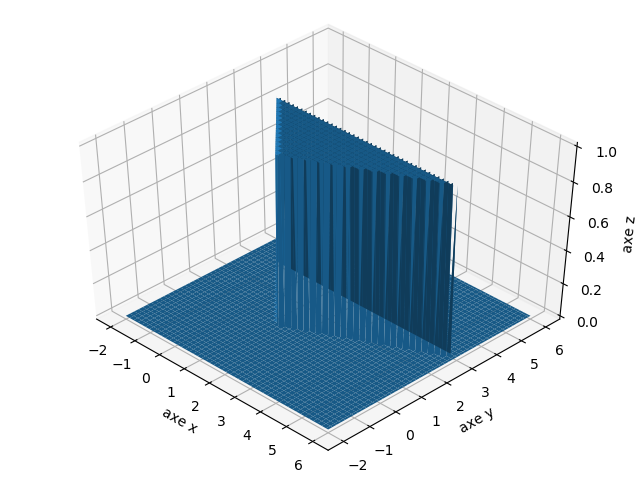
\includegraphics[scale=\myscale,scale=0.4]{figures/neurones-surface-2-heaviside}
Activation $H$
\end{minipage}\quad
\begin{minipage}{0.4\textwidth}
\center
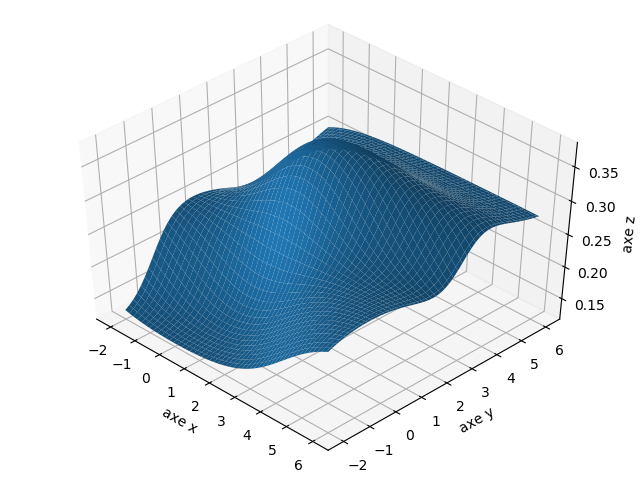
\includegraphics[scale=\myscale,scale=0.4]{figures/neurones-surface-2-sigma}
Activation $\sigma$
\end{minipage}
\end{center}

\begin{center}
\begin{minipage}{0.4\textwidth}
\center
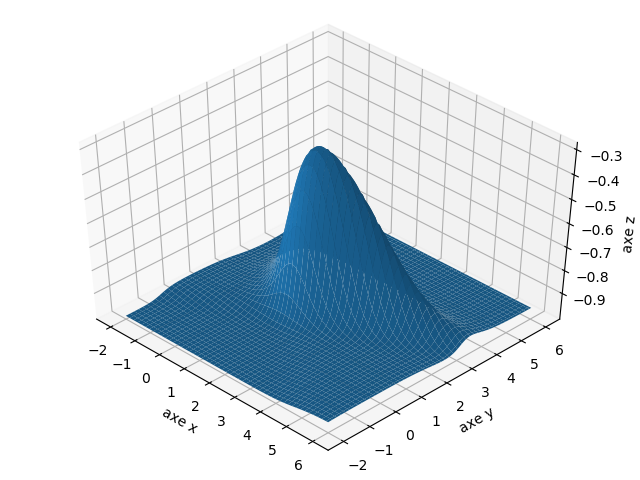
\includegraphics[scale=\myscale,scale=0.4]{figures/neurones-surface-2-tanh}
Activation $\tanh$
\end{minipage}\quad
\begin{minipage}{0.4\textwidth}
\center
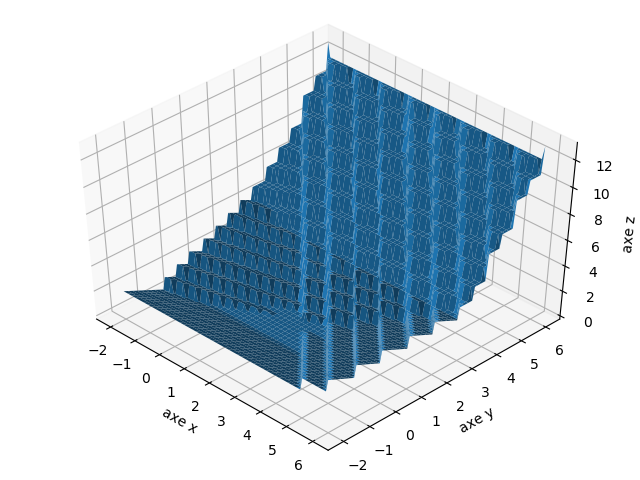
\includegraphics[scale=\myscale,scale=0.4]{figures/neurones-surface-2-relu}
Activation ReLU
\end{minipage}
\end{center}
\end{exemple}


% \todo{Exercice td : rond bleu, carrés rouge avec trois droites}


% \todo{Exercice td : l'influence d'un poids sur la fonction générée par le réseau. à faire réseau 2+1, H, un coeff qui varie, i.e. une droite varie plusieurs dessins}

%%%%%%%%%%%%%%%%%%%%%%%%%%%%%%%%%%%%%%%%%%%%%%%%%%%%%%%%%%%%%%%%%%%%%
\section{Théorie des réseaux de neurones}

%--------------------------------------------------------------------
\subsection{OU exclusif}

Nous avons vu qu'un seul neurone ne permet pas de réaliser la fonction associée au \og{}OU exclusif\fg{}.
Avec plusieurs neurones c'est facile !
Voici un réseau de neurones qui sépare le plan en trois parties, le secteur central en lequel la fonction associée au réseau vaut $0$, alors que la fonction vaut $1$ partout ailleurs (y compris sur la frontière\couleurnb{ rouge}).
\myfigure{0.7}{
\tikzinput{fig_neurones_54}
}

\myfigure{0.8}{
\tikzinput{fig_neurones_55}
}



Ce réseau permet d'obtenir une valeur $F(x,y)=1$ en $(1,0)$ et $(0,1)$ et une valeur $F(x,y)=0$ en $(0,0)$ et $(1,1)$.

L'idée de ce réseau vient du fait que l'opération \og{}OU exclusif\fg{} est une combinaison de \og{}OU\fg{} et de \og{}ET\fg{} :
$$x \text{ OUex } y  = (x \text{ ET } \text{non} y) \text{ OU } ( \text{non} x \text{ ET } y).$$


\begin{center}
\begin{minipage}{0.60\textwidth}
\myfigure{0.9}{
\tikzinput{fig_neurones_56}
}
\end{minipage}
\begin{minipage}{0.39\textwidth}
\myfigure{0.8}{
\tikzinput{fig_neurones_31}
}
\end{minipage}
\end{center}

Le neurone du haut réalise \og{}$x \text{ ET } \text{non} y$\fg{}, le neurone du bas \og{}$\text{non} x \text{ ET } y$\fg{} et celui de sortie l'opération \og{}OU\fg{}.

%--------------------------------------------------------------------
\subsection{Ensemble réalisable}

Nous aimerions savoir quels ensembles peuvent être décrits par un réseau de neurones.
On rappelle qu'un ensemble $A \subset \Rr^2$ découpe le plan en trois parties disjointes : intérieur, frontière, extérieur :
$$\Int(A) \qquad \Fr(A) \qquad \Ext(A).$$

\myfigure{0.9}{
\tikzinput{fig_neurones_57}
}

\begin{definition}
Un ensemble $A$ est dit \defi{réalisable par un réseau de neurones} s'il existe un réseau de neurones $\mathcal{R}$ (d'unique fonction d'activation la fonction marche de Heaviside) tel que
la fonction $F : \Rr^2 \to \Rr$ associée à $\mathcal{R}$ vérifie :
$$F(x,y) = 1 \quad \text{ pour tout } (x,y) \in \Int(A)$$
et
$$F(x,y) = 0 \quad \text{ pour tout } (x,y) \in \Ext(A).$$
\end{definition}

\myfigure{0.9}{
\tikzinput{fig_neurones_58}
}


Remarque : on n'exige rien sur la frontière $\Fr(A)$, $F$ peut y prendre la valeur $0$ ou la valeur $1$.


Voici les types d'ensembles que nous avons déjà réalisés :
\begin{itemize}
  \item les demi-plans,
  \item les \og{}quart de plans\fg{},
  \item les zones triangulaires,
  \item les triangles avec un sommet \og{}à l'infini\fg{}.
\end{itemize}

\myfigure{0.6}{
\tikzinput{fig_neurones_59}
}


En augmentant le nombre de neurones, on peut réaliser les quadrilatères convexes et plus généralement n'importe quelle zone polygonale convexe.

\begin{proposition}
Tout zone polygonale convexe à $n$ côtés est réalisable par un réseau de $n+1$ neurones.
\end{proposition}

\myfigure{0.6}{
\tikzinput{fig_neurones_60}
}

\begin{proof}
Un polygone convexe à $n$ côtés est l'intersection de $n$ demi-plans.
Chaque demi-plan, bordé par une droite d'équation du type $ax+by+c=0$, correspond à un neurone de la première couche dont les coefficients sont $(a,b)$ et le biais est $c$ (ou alors $(-a,-b)$ et $-c$).
Sur la seconde couche, on place un neurone qui réalise l'opération \og{}ET\fg{} sur les $n$ entrées : tous ses coefficients sont $1$ et le biais est $-n$.
\end{proof}

Continuons avec des opérations élémentaires sur les ensembles réalisables.
\begin{proposition}
Si $A$ et $B$ sont deux ensembles du plan réalisables par des réseaux de neurones alors :
$$A\cup B \qquad A\cap B \qquad A^\complement  \qquad A \setminus B$$
sont aussi des ensembles réalisables. 
\end{proposition}


\myfigure{0.8}{
\tikzinput{fig_neurones_61}
}


\begin{proof}
~
\begin{itemize}
  \item Si $A$ est réalisé par un réseau $\mathcal{R}_A$ et $B$ par un réseau  $\mathcal{R}_B$
alors on crée un nouveau réseau $\mathcal{R}$ en superposant $\mathcal{R}_A$ et $\mathcal{R}_B$
et en ajoutant un neurone \og{}OU\fg{} à partir des sorties de $\mathcal{R}_A$ et $\mathcal{R}_B$.
Ainsi si $(x,y)$ est dans $A \cup B$, il est dans $A$ ou dans $B$, une des sorties  $\mathcal{R}_A$ ou $\mathcal{R}_B$ vaut alors $1$ et le neurone sortant de $\mathcal{R}$ s'active.

\myfigure{0.8}{
\tikzinput{fig_neurones_62}
}


  \item Pour réaliser $A \cap B$, on remplace le neurone \og{}OU\fg{} par un neurone \og{}ET\fg{}.

\myfigure{0.8}{
\tikzinput{fig_neurones_63}
}

  \item Pour réaliser le complément d'un ensemble $A$, on utilise l'opération \og{}non\fg{} : $0$ s'envoie sur $1$ et $1$ sur $0$. Ceci se fait par l'application 
  $s \mapsto 1-s$. Il suffit juste de rajouter un neurone \og{}NON\fg{} à $\mathcal{R}_A$.
 
\myfigure{0.8}{
\tikzinput{fig_neurones_64}
} 
  
  \item Comme $A \setminus B = A \cap \big((A\cap B)^\complement \big)$ alors 
  il est possible de réaliser $A \setminus B$ comme succession d'opérations élémentaires $\cap$, $\complement$ et $\cup$.
\end{itemize}


\end{proof}

% [[Pb de la frontière? si $A$ réalisable alors $A\cup \Fr(A)$ *vraiment* réalisable et $A\setminus \Fr(A)$ aussi]]






\begin{proposition}
Tout polygone (convexe ou non) est réalisable par un réseau de neurones.
\end{proposition}

\begin{proof}
Un polygone peut être découpé en triangles. Chaque triangle est réalisable, donc l'union des triangles l'est aussi.

\myfigure{0.8}{
\tikzinput{fig_neurones_65}
}


\end{proof}

%--------------------------------------------------------------------
\subsection{Approximation d'ensembles}



On rappelle qu'une \defi{courbe de Jordan} $C$ est une courbe fermée simple (c'est l'image d'un cercle par une application continue injective). Le théorème suivant est une sorte de théorème d'approximation universelle géométrique.
\myfigure{0.8}{
\tikzinput{fig_neurones_66}
}

\begin{theoreme}
Un ensemble $A$ délimité par une courbe de Jordan peut être approché d'aussi près que l'on veut par un ensemble $A'$ réalisable par un réseau de neurones.
\end{theoreme}

Il s'agit juste du fait qu'une courbe de Jordan peut être approchée par un polygone.
C'est un résultat théorique qui ne dit en rien comment choisir la structure du réseau ou les poids.

\myfigure{0.8}{
\tikzinput{fig_neurones_67}
}

% [[Preuve voir Tverberg, A proof of the Jordan curve theorem, Bull London Math Soc, 1980]]



%%%%%%%%%%%%%%%%%%%%%%%%%%%%%%%%%%%%%%%%%%%%%%%%%%%%%%%%%%%%%%%%%%%%%
\section{Théorème d'approximation universelle}

Nous allons maintenant prouver qu'un réseau de neurones bien construit peut approcher n'importe quelle fonction. 

Dans cette section nous partirons d'une seule entrée $x \in \Rr$, avec une seule sortie $y = F(x) \in \Rr$. Les réseaux de neurones de cette section produisent donc des fonctions $F : \Rr \to \Rr$.

L'objectif est le suivant : on nous donne une fonction $f : [a,b] \to \Rr$ et nous devons trouver un réseau, tel que la fonction $F$ associée à ce réseau soit proche de $f$ :
$$F(x) \simeq f(x) \qquad \text{ pour tout } x \in [a,b].$$

Pour paramétrer le réseau nous allons bien sûr fixer des poids, mais avant cela choisissons les fonctions d'activation :
\begin{itemize}
  \item pour le neurone de sortie, on choisit la fonction identité $\phi(x)=x$,
  \item pour tous les autres neurones, on choisit la fonction marche de Heaviside.
\end{itemize}


\begin{remarque*}
\sauteligne
\begin{itemize}
  \item Si on choisissait aussi la fonction d'activation marche de Heaviside pour le neurone de sortie, alors $F$ ne pourrait prendre que deux valeurs, $0$ ou $1$, ce qui empêcherait de réaliser la plupart des fonctions.
  
  \item Par contre, si on choisissait la fonction identité pour tous les neurones alors on ne réaliserait que des fonctions affines $F(x)=ax+b$ (en effet la composition de plusieurs fonctions affines reste une fonction affine). 

\end{itemize}
\end{remarque*}

%--------------------------------------------------------------------
\subsection{Fonctions marches}
\label{ssec:marches}

Nous allons réaliser des fonctions de plus en plus compliquées à partir d'éléments très simples.


Commençons par étudier le comportement d'un seul neurone avec la fonction d'activation marche de Heaviside (on rajoutera le neurone de sortie plus tard).

Voici différents neurones et les fonctions qu'ils réalisent :
\begin{itemize}
  \item La fonction marche de Heaviside.
  
\begin{center}
\begin{minipage}{0.35\textwidth}
\myfigure{0.9}{
\tikzinput{fig_neurones_68}
}
\end{minipage}
\begin{minipage}{0.59\textwidth}
\myfigure{0.7}{
\tikzinput{fig_neurones_69}
}
\end{minipage}
\end{center}  

  
\item La fonction marche décalée vers la gauche, avec $a>0$.
  
Preuve : $F(x) = 1 \iff ax+1\ge0 \iff x \ge -\frac1a$.
  
\begin{center}
\begin{minipage}{0.35\textwidth}
\myfigure{0.9}{
\tikzinput{fig_neurones_70}
}
\end{minipage}
\begin{minipage}{0.59\textwidth}
\myfigure{0.7}{
\tikzinput{fig_neurones_71}
}
\end{minipage}
\end{center}    
    
  \item La fonction marche décalée vers la droite, avec $a>0$.  
  
\begin{center}
\begin{minipage}{0.35\textwidth}
\myfigure{0.9}{
\tikzinput{fig_neurones_72}
}
\end{minipage}
\begin{minipage}{0.59\textwidth}
\myfigure{0.7}{
\tikzinput{fig_neurones_73}
}
\end{minipage}
\end{center}    

  
\item La fonction marche à l'envers décalée vers la droite, avec $b>0$.
  
  Preuve : $F(x) = 1 \iff -bx+1\ge0 \iff bx \le 1 \iff x \le \frac1b$.
  
\begin{center}
\begin{minipage}{0.35\textwidth}
\myfigure{0.9}{
\tikzinput{fig_neurones_74}
}
\end{minipage}
\begin{minipage}{0.59\textwidth}
\myfigure{0.7}{
\tikzinput{fig_neurones_75}
}
\end{minipage}
\end{center}  
  

  \item La fonction marche à l'envers décalée vers la gauche, avec $b>0$.  
  
\begin{center}
\begin{minipage}{0.35\textwidth}
\myfigure{0.9}{
\tikzinput{fig_neurones_76}
}
\end{minipage}
\begin{minipage}{0.59\textwidth}
\myfigure{0.7}{
\tikzinput{fig_neurones_77}
}
\end{minipage}
\end{center}   
\end{itemize}

Selon les cas, la valeur au niveau de la marche est $0$ ou $1$. On peut obtenir l'autre situation en rajoutant un neurone de type \og{}NON\fg{}.

\begin{center}
\begin{minipage}{0.35\textwidth}
\myfigure{0.9}{
\tikzinput{fig_neurones_78}
}
\end{minipage}
\begin{minipage}{0.59\textwidth}
\myfigure{0.7}{
\tikzinput{fig_neurones_79}
}
\end{minipage}
\end{center}  



%--------------------------------------------------------------------
\subsection{Fonctions créneaux}

Pour réaliser un \og{}créneau\fg{}, l'idée est d'additionner une marche à l'endroit et une marche à l'envers.

\myfigure{0.7}{
\tikzinput{fig_neurones_80}
}

Pour effectuer cette opération, nous allons construire un réseau avec deux neurones sur la première couche (de fonction d'activation $H$) et un neurone sur la seconde couche (de fonction d'activation identité) qui additionne les deux sorties précédentes et soustrait $1$ (afin de ramener la ligne de base à $0$).

\begin{center}
\begin{minipage}{0.55\textwidth}
\myfigure{0.9}{
\tikzinput{fig_neurones_81}
}
\end{minipage}
\begin{minipage}{0.35\textwidth}
\myfigure{0.7}{
\tikzinput{fig_neurones_82}
}
\end{minipage}
\end{center}  


Si on veut une marche plus haute il suffit de changer les poids du neurone de sortie d'un facteur $k$.

\begin{center}
\begin{minipage}{0.55\textwidth}
\myfigure{0.9}{
\tikzinput{fig_neurones_83}
}
\end{minipage}
\begin{minipage}{0.35\textwidth}
\myfigure{0.7}{
\tikzinput{fig_neurones_84}
}
\end{minipage}
\end{center} 

%--------------------------------------------------------------------
\subsection{Fonctions en escalier}
On réalise des doubles créneaux en superposant les premières couches de chaque créneau et en réunissant les deux neurones de sortie. Voici un exemple avec un créneau de hauteur $4$ sur $[2,3]$ et un créneau de hauteur $6$ sur $[5,10]$.

\begin{center}
\begin{minipage}{0.50\textwidth}
\myfigure{0.8}{
\tikzinput{fig_neurones_85}
}
\end{minipage}
\begin{minipage}{0.45\textwidth}
\myfigure{0.5}{
\tikzinput{fig_neurones_86}
}
\end{minipage}
\end{center} 


On peut aussi calculer la valeur de la fonction $F$ de la façon suivante ($s_i$ représente la sortie du neurone numéro $i$ de la première couche) :
$$F(x) = \underbrace{4s_1+4s_2-4}_{\text{vaut $4$ ou $0$}} + \underbrace{6s_3+6s_4-6}_{\text{vaut $6$ ou $0$}} = 
\begin{cases}
4 & \text{ si } x \in [2,3[ \\
6 & \text{ si } x \in [5,10[ \\
0 & \text {sinon}
\end{cases}
$$

\begin{remarque*}
\sauteligne
\begin{itemize}
  \item Noter l'écriture avec deux biais $-4$ et $-6$ pour le neurone de sortie. C'est juste une écriture pour décomposer et expliquer le \og{}vrai\fg{} biais qui est $-4-6 = -10$.

  \item Il peut y avoir un problème pour réaliser deux créneaux contigus. Si on n'y prend pas garde, la valeur est mauvaise à la jonction (c'est la somme des deux valeurs). Pour corriger le problème, il faut utiliser une marche où on a changé la valeur au bord, voir la fin de la section \ref{ssec:marches}.
  
  \myfigure{0.6}{
  \tikzinput{fig_neurones_87}
  }
 
\end{itemize}
\end{remarque*} 

Une \defi{fonction en escalier} est une fonction qui est constante sur un nombre fini d'intervalles bornés.


  \myfigure{1.1}{
  \tikzinput{fig_neurones_88}
  }


\begin{proposition}
Toute fonction en escalier est réalisable par un réseau de neurones.
\end{proposition}

\begin{proof}
Soit $n$ le nombre de marches de l'escalier.
On construit un réseau de $2n+1$ neurones. La première couche est constituée de $n$ paires de neurones, chaque paire réalise une marche de l'escalier. La seconde couche contient uniquement le neurone de sortie, les coefficients sont choisis pour ajuster la hauteur de la marche et le biais assure que la fonction vaut $0$ en dehors de l'escalier.

Si on veut les valeurs exactes aux bornes des marches, il faut éventuellement ajouter des neurones de type \og{}NON\fg{} entre la première couche et le neurone de sortie.
\end{proof}

%--------------------------------------------------------------------
\subsection{Théorème d'approximation universelle (une variable)}

\index{theoreme@théorème d'approximation universelle}

Nous pouvons maintenant énoncer le résultat théorique le plus important de ce chapitre.

\begin{theoreme}[Théorème d'approximation universelle]
Toute fonction continue $f : [a,b] \to \Rr$ peut être approchée d'aussi près que l'on veut par une fonction $F : [a,b] \to \Rr$ réalisée par un réseau de neurones.
\end{theoreme}

Plusieurs commentaires importants.
\begin{itemize}
  \item Tout d'abord rappelons que nous réalisons nos neurones avec des fonctions d'activation $H$ (marche de Heaviside) sauf pour le neurone de sortie qui a pour fonction d'activation l'identité.
  
  \item Les hypothèses sont importantes : $f$ est continue et définie sur un intervalle fermé et borné. Si une des hypothèses venait à manquer l'énoncé serait faux.
  
  \item Bien que l'énoncé ne le dise pas, on peut concrètement réaliser à la main un réseau qui approche la fonction $f$ (voir le chapitre suivant). Cependant, ce n'est pas l'esprit des réseaux de neurones.
  
  \item Que signifie \og{}approcher d'aussi près que l'on veut la fonction $f$\fg{} ? C'est dire que pour chaque $\epsilon>0$, il existe une fonction $F$ (ici issue d'un réseau de neurones), telle que :
  $$\text{pour tout } x \in [a,b] \qquad | f(x)-F(x) | < \epsilon.$$
  C'est l'\defi{approximation uniforme} des fonctions.
  
\end{itemize}


\begin{proof}  
La preuve est simple : toute fonction continue sur un intervalle $[a,b]$ peut être approchée d'aussi près que l'on veut par une fonction en escalier. Par exemple, on subdivise l'intervalle $[a,b]$ en $n$ sous-intervalles $[x_i,x_{i+1}]$ et on prend une marche de hauteur $f(x_i)$ sur cet intervalle. Comme nous avons prouvé que l'on sait réaliser toutes les fonctions en escalier, la preuve est terminée.

  \myfigure{1}{
  \tikzinput{fig_neurones_89}
  }


\end{proof}
  
Remarque : la preuve se rapproche de la construction de l'intégrale. Pour calculer l'intégrale, on calcule en fait l'aire de rectangles. Ces rectangles correspondent à nos fonctions en escalier. 


%--------------------------------------------------------------------
\subsection{Théorème d'approximation universelle (deux variables et plus)}

Ce que nous avons fait pour une variable, nous pouvons le faire pour deux variables (ou plus).

\begin{theoreme}[Théorème d'approximation universelle]
Toute fonction continue $f : [a,b]\times [a,b] \to \Rr$ peut être approchée d'aussi près que l'on veut par une fonction $F : [a,b]\times [a,b] \to \Rr$ réalisée par un réseau de neurones.
\end{theoreme}

Il suffit là encore de réaliser des fonctions marches élémentaires. Nous ne donnons pas de détails mais seulement l'exemple d'un réseau qui réalise la fonction
$F : \Rr^2 \to \Rr$ qui vaut $1$ sur $[0,1]\times [0,1]$ et $0$ partout ailleurs.


\myfigure{0.95}{
\tikzinput{fig_neurones_90}
}



\begin{center}
\begin{minipage}{0.45\textwidth}
\myfigure{1}{\tikzinput{fig_neurones_91}}
\end{minipage}
\begin{minipage}{0.45\textwidth}
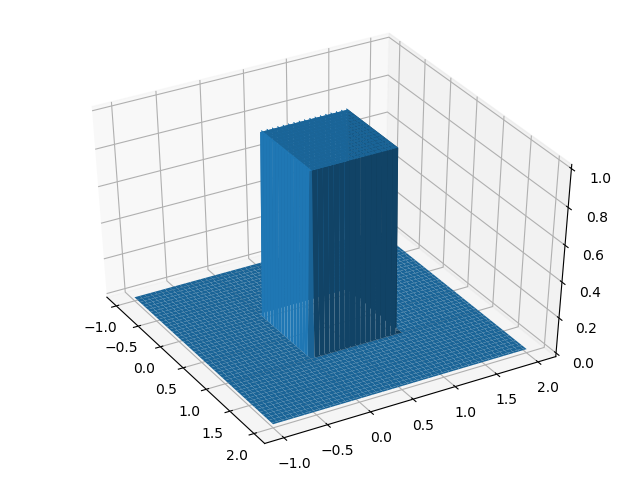
\includegraphics[scale=\myscale,scale=0.5]{figures/neurones-surface-1}
\end{minipage}
\end{center}


\end{document}
